\documentclass{standalone}
\usepackage{tikz}
\usetikzlibrary{patterns, positioning}


\begin{document}
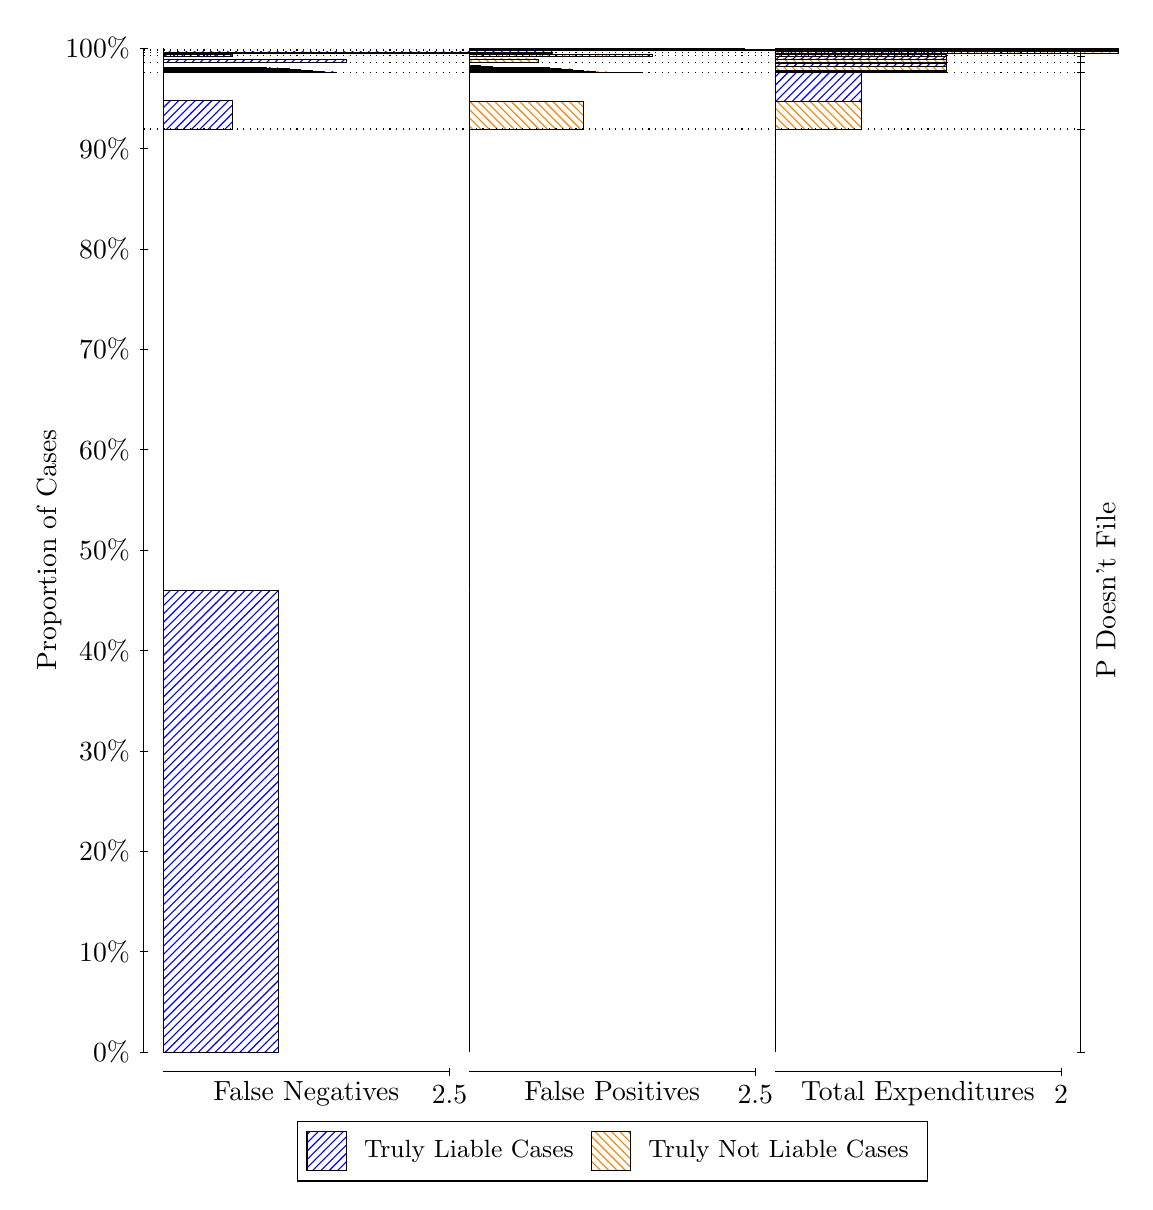
\begin{tikzpicture}
\draw[black, very thin] (1.5,1.75) -- (1.5,14.5);
\node[rotate=90, text=black, anchor=center] at (0.3, 8.125) {Proportion of Cases};
\draw[black, very thin] (1.45,1.75) -- (1.55,1.75);
\node[text=black, anchor=east] at (1.45, 1.75) {0\%};
\draw[black, very thin] (1.45,3.025) -- (1.55,3.025);
\node[text=black, anchor=east] at (1.45, 3.025) {10\%};
\draw[black, very thin] (1.45,4.3) -- (1.55,4.3);
\node[text=black, anchor=east] at (1.45, 4.3) {20\%};
\draw[black, very thin] (1.45,5.575) -- (1.55,5.575);
\node[text=black, anchor=east] at (1.45, 5.575) {30\%};
\draw[black, very thin] (1.45,6.85) -- (1.55,6.85);
\node[text=black, anchor=east] at (1.45, 6.85) {40\%};
\draw[black, very thin] (1.45,8.125) -- (1.55,8.125);
\node[text=black, anchor=east] at (1.45, 8.125) {50\%};
\draw[black, very thin] (1.45,9.4) -- (1.55,9.4);
\node[text=black, anchor=east] at (1.45, 9.4) {60\%};
\draw[black, very thin] (1.45,10.675) -- (1.55,10.675);
\node[text=black, anchor=east] at (1.45, 10.675) {70\%};
\draw[black, very thin] (1.45,11.95) -- (1.55,11.95);
\node[text=black, anchor=east] at (1.45, 11.95) {80\%};
\draw[black, very thin] (1.45,13.225) -- (1.55,13.225);
\node[text=black, anchor=east] at (1.45, 13.225) {90\%};
\draw[black, very thin] (1.45,14.5) -- (1.55,14.5);
\node[text=black, anchor=east] at (1.45, 14.5) {100\%};

\draw[black, very thin] (13.4,1.75) -- (13.4,14.5);
\draw[black, very thin] (13.35,1.75) -- (13.45,1.75);
\node[anchor=west] at (13.35, 1.75) {};
\draw[black, very thin] (13.35,13.472) -- (13.45,13.472);
\node[anchor=west] at (13.35, 13.472) {};
\draw[black, very thin] (13.35,14.187) -- (13.45,14.187);
\node[anchor=west] at (13.35, 14.187) {};
\draw[black, very thin] (13.35,14.32) -- (13.45,14.32);
\node[anchor=west] at (13.35, 14.32) {};
\draw[black, very thin] (13.35,14.401) -- (13.45,14.401);
\node[anchor=west] at (13.35, 14.401) {};
\draw[black, very thin] (13.35,14.438) -- (13.45,14.438);
\node[anchor=west] at (13.35, 14.438) {};
\draw[black, very thin] (13.35,14.475) -- (13.45,14.475);
\node[anchor=west] at (13.35, 14.475) {};
\draw[black, very thin] (13.35,14.5) -- (13.45,14.5);
\node[anchor=west] at (13.35, 14.5) {};

\draw[black, very thin, pattern color=blue, pattern=north east lines] (1.75,1.75) rectangle (3.2033,7.6112);
\draw[black, very thin, pattern color=orange, pattern=north west lines] (1.75,7.6112) rectangle (1.75,13.472);
\draw[black, very thin, pattern color=blue, pattern=north east lines] (1.75,13.472) rectangle (2.622,13.832);
\draw[black, very thin, pattern color=orange, pattern=north west lines] (1.75,13.832) rectangle (1.75,14.187);
\draw[black, very thin, pattern color=blue, pattern=north east lines] (1.75,14.187) rectangle (3.93,14.198);
\draw[black, very thin, pattern color=blue, pattern=north east lines] (1.75,14.198) rectangle (3.7847,14.203);
\draw[black, very thin, pattern color=blue, pattern=north east lines] (1.75,14.203) rectangle (3.6393,14.218);
\draw[black, very thin, pattern color=blue, pattern=north east lines] (1.75,14.218) rectangle (3.494,14.231);
\draw[black, very thin, pattern color=blue, pattern=north east lines] (1.75,14.231) rectangle (3.3487,14.245);
\draw[black, very thin, pattern color=blue, pattern=north east lines] (1.75,14.245) rectangle (3.2033,14.248);
\draw[black, very thin, pattern color=blue, pattern=north east lines] (1.75,14.248) rectangle (3.058,14.252);
\draw[black, very thin, pattern color=blue, pattern=north east lines] (1.75,14.252) rectangle (2.9127,14.253);
\draw[black, very thin, pattern color=blue, pattern=north east lines] (1.75,14.253) rectangle (2.7673,14.255);
\draw[black, very thin, pattern color=orange, pattern=north west lines] (1.75,14.255) rectangle (1.75,14.32);
\draw[black, very thin, pattern color=blue, pattern=north east lines] (1.75,14.32) rectangle (4.0753,14.358);
\draw[black, very thin, pattern color=orange, pattern=north west lines] (1.75,14.358) rectangle (1.75,14.401);
\draw[black, very thin, pattern color=blue, pattern=north east lines] (1.75,14.401) rectangle (2.622,14.421);
\draw[black, very thin, pattern color=orange, pattern=north west lines] (1.75,14.421) rectangle (1.75,14.438);
\draw[black, very thin, pattern color=blue, pattern=north east lines] (1.75,14.438) rectangle (6.6913,14.452);
\draw[black, very thin, pattern color=orange, pattern=north west lines] (1.75,14.452) rectangle (1.75,14.475);
\draw[black, very thin, pattern color=orange, pattern=north west lines] (1.75,14.475) rectangle (1.75,14.485);
\draw[black, very thin, pattern color=blue, pattern=north east lines] (1.75,14.485) rectangle (1.75,14.5);
\draw[black, very thin, pattern color=orange, pattern=north west lines] (5.6333,1.75) rectangle (5.6333,7.6112);
\draw[black, very thin, pattern color=blue, pattern=north east lines] (5.6333,7.6112) rectangle (5.6333,13.472);
\draw[black, very thin, pattern color=orange, pattern=north west lines] (5.6333,13.472) rectangle (7.0867,13.827);
\draw[black, very thin, pattern color=blue, pattern=north east lines] (5.6333,13.827) rectangle (5.6333,14.187);
\draw[black, very thin, pattern color=orange, pattern=north west lines] (5.6333,14.187) rectangle (7.8133,14.188);
\draw[black, very thin, pattern color=orange, pattern=north west lines] (5.6333,14.188) rectangle (7.668,14.19);
\draw[black, very thin, pattern color=orange, pattern=north west lines] (5.6333,14.19) rectangle (7.5227,14.193);
\draw[black, very thin, pattern color=orange, pattern=north west lines] (5.6333,14.193) rectangle (7.3773,14.197);
\draw[black, very thin, pattern color=orange, pattern=north west lines] (5.6333,14.197) rectangle (7.232,14.209);
\draw[black, very thin, pattern color=orange, pattern=north west lines] (5.6333,14.209) rectangle (7.0867,14.22);
\draw[black, very thin, pattern color=orange, pattern=north west lines] (5.6333,14.22) rectangle (6.9413,14.234);
\draw[black, very thin, pattern color=orange, pattern=north west lines] (5.6333,14.234) rectangle (6.796,14.239);
\draw[black, very thin, pattern color=orange, pattern=north west lines] (5.6333,14.239) rectangle (6.6507,14.253);
\draw[black, very thin, pattern color=blue, pattern=north east lines] (5.6333,14.253) rectangle (6.36,14.254);
\draw[black, very thin, pattern color=blue, pattern=north east lines] (5.6333,14.254) rectangle (6.2147,14.256);
\draw[black, very thin, pattern color=blue, pattern=north east lines] (5.6333,14.256) rectangle (6.0693,14.259);
\draw[black, very thin, pattern color=blue, pattern=north east lines] (5.6333,14.259) rectangle (5.924,14.262);
\draw[black, very thin, pattern color=blue, pattern=north east lines] (5.6333,14.262) rectangle (5.7787,14.276);
\draw[black, very thin, pattern color=blue, pattern=north east lines] (5.6333,14.276) rectangle (5.6333,14.32);
\draw[black, very thin, pattern color=orange, pattern=north west lines] (5.6333,14.32) rectangle (6.5053,14.363);
\draw[black, very thin, pattern color=blue, pattern=north east lines] (5.6333,14.363) rectangle (5.6333,14.401);
\draw[black, very thin, pattern color=orange, pattern=north west lines] (5.6333,14.401) rectangle (7.9587,14.418);
\draw[black, very thin, pattern color=blue, pattern=north east lines] (5.6333,14.418) rectangle (6.5053,14.438);
\draw[black, very thin, pattern color=orange, pattern=north west lines] (5.6333,14.438) rectangle (5.6333,14.461);
\draw[black, very thin, pattern color=blue, pattern=north east lines] (5.6333,14.461) rectangle (5.6333,14.475);
\draw[black, very thin, pattern color=orange, pattern=north west lines] (5.6333,14.475) rectangle (10.575,14.485);
\draw[black, very thin, pattern color=blue, pattern=north east lines] (5.6333,14.485) rectangle (9.1213,14.5);
\draw[black, very thin, pattern color=orange, pattern=north west lines] (9.5167,1.75) rectangle (9.5167,7.6112);
\draw[black, very thin, pattern color=blue, pattern=north east lines] (9.5167,7.6112) rectangle (9.5167,13.472);
\draw[black, very thin, pattern color=orange, pattern=north west lines] (9.5167,13.472) rectangle (10.607,13.827);
\draw[black, very thin, pattern color=blue, pattern=north east lines] (9.5167,13.827) rectangle (10.607,14.187);
\draw[black, very thin, pattern color=orange, pattern=north west lines] (9.5167,14.187) rectangle (11.697,14.199);
\draw[black, very thin, pattern color=blue, pattern=north east lines] (9.5167,14.199) rectangle (11.697,14.213);
\draw[black, very thin, pattern color=orange, pattern=north west lines] (9.5167,14.213) rectangle (11.697,14.262);
\draw[black, very thin, pattern color=blue, pattern=north east lines] (9.5167,14.262) rectangle (11.697,14.311);
\draw[black, very thin, pattern color=orange, pattern=north west lines] (9.5167,14.311) rectangle (11.697,14.315);
\draw[black, very thin, pattern color=blue, pattern=north east lines] (9.5167,14.315) rectangle (11.697,14.32);
\draw[black, very thin, pattern color=orange, pattern=north west lines] (9.5167,14.32) rectangle (11.697,14.363);
\draw[black, very thin, pattern color=blue, pattern=north east lines] (9.5167,14.363) rectangle (11.697,14.401);
\draw[black, very thin, pattern color=orange, pattern=north west lines] (9.5167,14.401) rectangle (11.697,14.418);
\draw[black, very thin, pattern color=blue, pattern=north east lines] (9.5167,14.418) rectangle (11.697,14.438);
\draw[black, very thin, pattern color=orange, pattern=north west lines] (9.5167,14.438) rectangle (13.877,14.461);
\draw[black, very thin, pattern color=blue, pattern=north east lines] (9.5167,14.461) rectangle (13.877,14.475);
\draw[black, very thin, pattern color=orange, pattern=north west lines] (9.5167,14.475) rectangle (13.877,14.485);
\draw[black, very thin, pattern color=blue, pattern=north east lines] (9.5167,14.485) rectangle (13.877,14.5);
\draw[black, dotted] (1.5,13.472) -- (13.4,13.472);
\draw[black, dotted] (1.5,14.187) -- (13.4,14.187);
\draw[black, dotted] (1.5,14.32) -- (13.4,14.32);
\draw[black, dotted] (1.5,14.401) -- (13.4,14.401);
\draw[black, dotted] (1.5,14.438) -- (13.4,14.438);
\draw[black, dotted] (1.5,14.475) -- (13.4,14.475);
\draw[black, very thin] (1.75,1.5) -- (5.3833,1.5);
\node[text=black, anchor=north] at (3.5667, 1.5) {False Negatives};
\draw[black, very thin] (5.3833,1.45) -- (5.3833,1.55);
\node[text=black, anchor=north] at (5.3833, 1.45) {2.5};

\draw[black, very thin] (5.6333,1.5) -- (9.2667,1.5);
\node[text=black, anchor=north] at (7.45, 1.5) {False Positives};
\draw[black, very thin] (9.2667,1.45) -- (9.2667,1.55);
\node[text=black, anchor=north] at (9.2667, 1.45) {2.5};

\draw[black, very thin] (9.5167,1.5) -- (13.15,1.5);
\node[text=black, anchor=north] at (11.333, 1.5) {Total Expenditures};
\draw[black, very thin] (13.15,1.45) -- (13.15,1.55);
\node[text=black, anchor=north] at (13.15, 1.45) {2};

\node[text=black, centered, rotate=90] at (13.72, 7.6112) {P Doesn't File};







\draw (7.449999999999999,1.5) node[draw=none] (baseCoordinate) {};
\begin{scope}[align=center]
        \matrix[scale=0.5, draw=black, below=0.5cm of baseCoordinate, nodes={draw}, column sep=0.1cm]{
            \node[rectangle, draw, minimum width=0.5cm, minimum height=0.5cm, pattern color=blue, pattern=north east lines] {}; &
            \node[draw=none, font=\small, text=black] (B) {Truly Liable Cases}; &
            \node[rectangle, draw, minimum width=0.5cm, minimum height=0.5cm, pattern color=orange, pattern=north west lines] {}; &
            \node[draw=none, font=\small, text=black] (B) {Truly Not Liable Cases}; \\
            };
\end{scope}

\end{tikzpicture}
\end{document}